\chapter{Evaluation}
\label{cha:evaluation}

\section{No Trailer, Generation Count of 50}
\label{sec:no_trailer_50}

In the following chapter we will compare the results, that is the path rating, and the required computation time for several different versions of the genetic algorithm.
Since there are many values and functions within the GA that can be adjusted and influence its performance, only a few can be considered here. The conclusion drawn in the next chapter \ref{cha:conclusion} will be based on the evaluation here.

The following table shows the rating achieved (higher is better) as well as the time needed for computation (lower is better) for several different setups of the algorithm. For each setup 7 runs and an average is given. Only the choice in GA functions used is changed between different runs, the remaining settings are consistent throughout the table and are as follows.

The population size is 1000, the algorithm runs for 50 generations and has a crossover rate of 60\%, a mutation rate of 0.1\% and the algorithm works without reordering operation. It starts at 175,350 and the destination is 740,100 (both are the program's default values). The vehicle has no trailers, an M value of 24,55, an L value of 42,5, and a starting angle of 45°, these values have been randomly generated and were then kept throughout all test runs.
Computation was done on a Core2Quad 6600@2.4GHz with 4GB of System Memory.

\begin{center}
	\begin{tabular}{| l | l | l | p{3cm} | p{3cm}|}
		\hline
		Run 		& 8Bit, Tournament 	& 8Bit, Roulette 	& TwoPoint, Tournament 	& TwoPoint, Roulette	\\ \hline
		1				&	152 in 1:50				&	222 in 1:44			&	647 in 1:53						&	49 in 1:57					\\ \hline
		2				&	90 in 1:47				&	134 in 1:51			& 111 in 154 \ref{pic:example_good_path}			&	127 in 2:01 \ref{pic:example_problem_path}	\\ \hline		
		3				&	127 in 1:48				&	106 in 1:54			& 240 in 1:48						& 51 in 1:58					\\ \hline
		4				&	240 in :144				&	61 in 1:46			& 122 in 1:48						& 130 in 2:01					\\ \hline
		5				&	152 in 1:49				&	222 in 1:57			&	274 in 1:49						&	156 in 1:54					\\ \hline
		6				&	163 in 1:49				& 201 in 1:56			&	56 in 1:57						& 78 in 1:51					\\ \hline
		7				&	90 in 2:06				&	76 in 1:53			& 59 in 1:47						& 230 in 1:56					\\ \hline
		Best		&	240 in 1:44				&	222 in 1:44			&	647 in 1:53						&	156 in 1:54					\\ \hline
		Worst		&	90 in 2:06				&	61 in 1:46			&	56 in 1:57						& 49 in 1:57					\\ \hline
		Average	&	144 in 1:51				& 146 in 1:51			& 198 in 1:50						&	117 in 1:56					\\ \hline
		\hline
	\end{tabular}
\end{center}


As can be seen from these results, the time is relatively consistent at just below 2 minutes. This of course depends heavily on the hardware used, but surprisingly very little on the oprations chosen within the GA. The results are not quite as consistent and have to be handled carefully due to the small sample size. Row 3 (TowPointCrossover, TournamentSelection) seems to deliver the best result, but this is largely due to a single very good path, which can be attributed to "`luck"' in the randomly generated path. If we disregard this single path we get an average of 143, which is almost the same as in the first two rows. The last row (TwoPointCrossover, RouletteWheelSelection) however produced sub-optimal paths rather consistently. It is also noticable that the difference between the best and worst path is much smaller in the first row when compared to the other three, which is why this setting has been chosen as the default one as it produces an acceptzable quality of paths rather consitently. These results may of course change with a (much) larger sample sizes.
The overall quality of the paths is rather low, which we will try to mitigate by raising the generation count in the next test, the real cause for this however is probably the rather primitive fitness function, see \ref{cha:conclusion} for further discussion. Right now the algorithm depends heavily on its initial random paths which leads to very different and overall sub-optimal results.
Two interesting paths are given in fig. \ref{pic:example_good_path} and fig. \ref{pic:example_problem_path}. Here, red is the path planned by the GA and blue is the actual, driveable, path obtained via simulation. In fig \ref{pic:example_good_path} we see an example of a good path which avoids all obstacles and gets very close to the target position. Whether or not it also hits the target configuration is not considered by the current fitness function. The path got a rating of 111, which is rather low compared to the ratings of some of the other, objectively worse, paths, which also points to the fitness function as the algorithms current weakness. \ref{pic:example_problem_path} shows a different problem with the current evaluation as it shows a path with a good rating (127) which also seems fine for the most part, but is completely impossible in reality as it passes through a wall. The current collision detection gives a worse rating the "`longer"' the path stays within the black area, which means that crossing a thin wall like this doesn't lower the rating by a whole lot compared to the positive rating it receives from the distance evaluation, even though the path is obvisouly still unusable. The current evaluation emphasizes distance to the target over the collision detection in order to obtain more acceptable paths quickly, but further optimization is required to make sure this does not come at the cost of accepting impossible paths.

\begin{figure}[h]
\centering
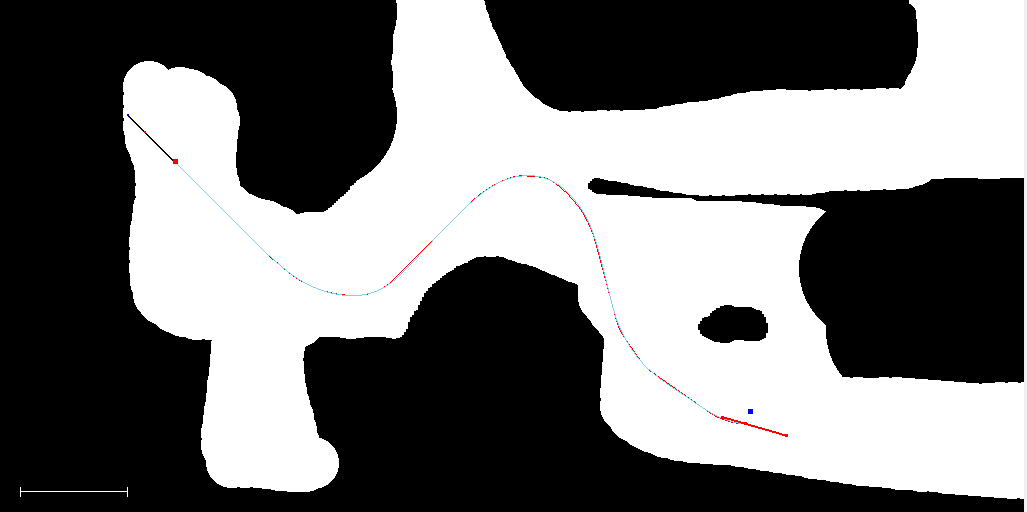
\includegraphics[width=0.75\textwidth]{./Chapters/Figures/example_good_path.png}
\caption{Example of a good result computed by the GA\label{pic:example_good_path}}
\end{figure}

\begin{figure}[h]
\centering
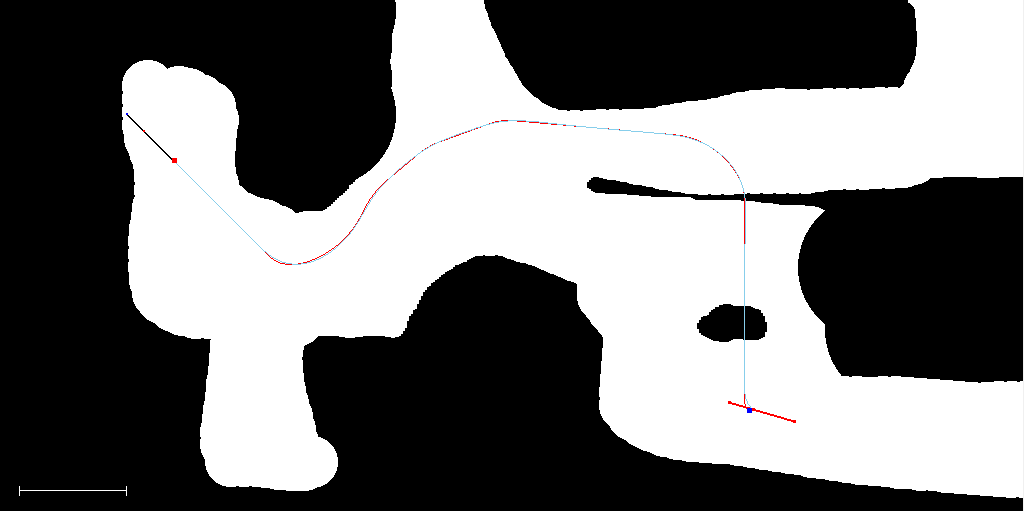
\includegraphics[width=0.75\textwidth]{./Chapters/Figures/example_problem_path.png}
\caption{A bad path with a good rating produced by the GA\label{pic:example_problem_path}}
\end{figure}

\begin{figure}[b]
\centering
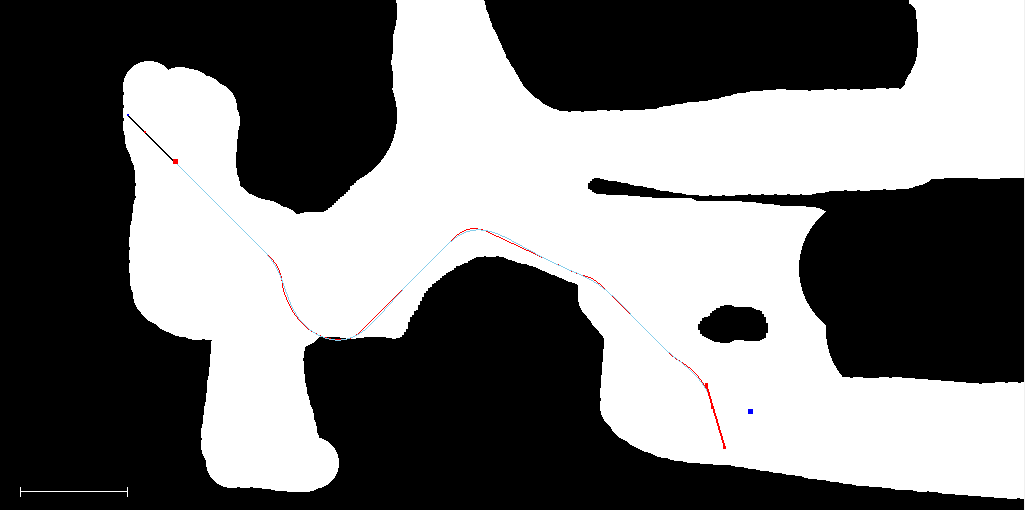
\includegraphics[width=0.75\textwidth]{./Chapters/Figures/example_problem_path2.png}
\caption{Another bad path with a good rating produced by the GA\label{pic:example_problem_path2}}
\end{figure}

\begin{figure}[b]
\centering
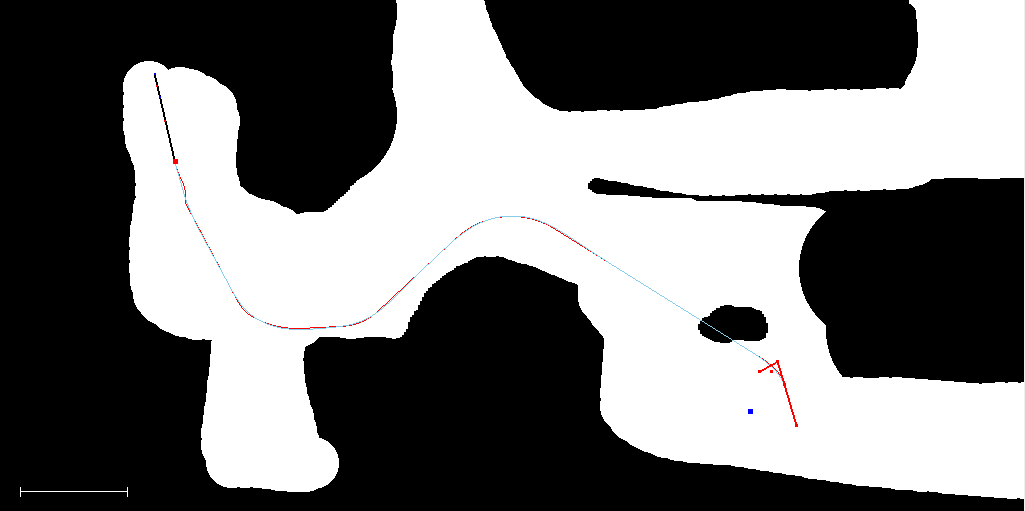
\includegraphics[width=0.75\textwidth]{./Chapters/Figures/example_good_path_trailer.png}
\caption{A (problem) path for a vehicle with one trailer.\label{pic:example_good_path_trailer}}
\end{figure}

\begin{figure}[b]
\centering
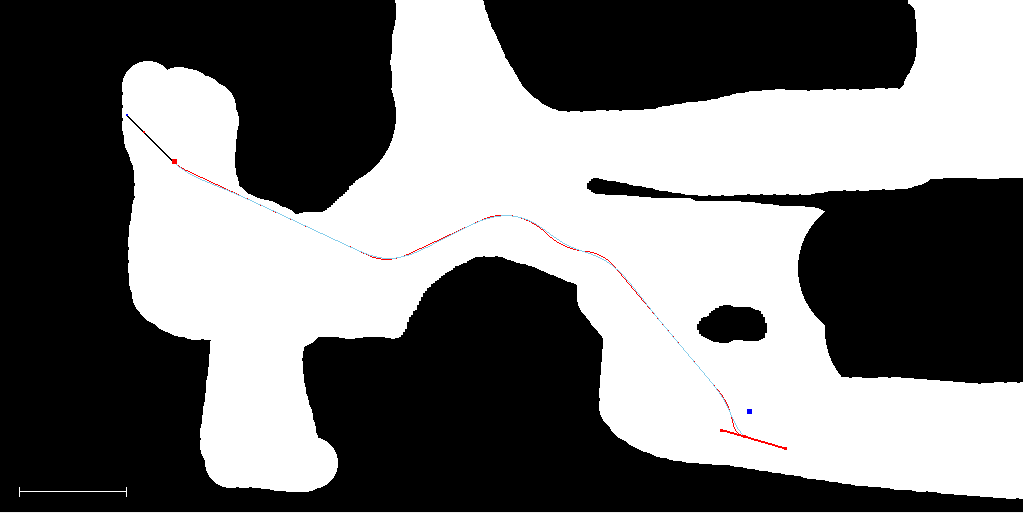
\includegraphics[width=0.75\textwidth]{./Chapters/Figures/example_good_path2.png}
\caption{Another example of a good result computed by the GA\label{pic:example_good_path2}}
\end{figure}


\section{No Trailer, Generation Count of 100}
\label{sec:no_trailer_100}

The settings in the following table are the exact same as in the previous ones, but the generation count has doubled to 100.
Due to time constraints, all evaluations after this points were done on a i5-M460@2,53 GHz instead of the Q6600 stated above. For comparison, the computation of the above table took an average of around 1:25, the same as in \ref{sec:no_trailer_50}, so about 25 seconds faster. Since, as we will see, the addition of a trailer does not impede the speed algoithm, we can simply make comparisons using \ref{sec:no_trailer_50}.

\begin{center}
	\begin{tabular}{| l | l | l | p{3cm} | p{3cm}|}
		\hline
		Run 		& 8Bit, Tournament 	& 8Bit, Roulette 	& TwoPoint, Tournament 	& TwoPoint, Roulette	\\ \hline
		1				291 in 2:44					&	146 in 2:33			&	73 in 2:38						&	93 in 2:37					\\ \hline
		2				&	138 in 2:36				&	143 in 2:35			&	175 in 2:38						&	56 in 2:38					\\ \hline
		3				&	235 in 2:35				&	194 in 2:41			&	123 in 2:37						&	48 in 2:39					\\ \hline
		4				&	109 in 2:35				&	65 in 2:42			&	105 in 2:47						&	78 in 2:36					\\ \hline
		5				&	191 in 2:39				&	101 in 2:38			&	539 in 2:36						&	69 in 2:41					\\ \hline
		6				&	259 in 2:48				&	148 in 2:39			&	211 in 2:36						&	180 in 2:36					\\ \hline
		7				&	67 in 2:43				&	156 in 2:35			&	136 in 2:37						&	166 in 2:38					\\ \hline
		Best		&	291 in 2:44				&	194 in 2:41			&	539 in 2:63						&	180 in 2:36					\\ \hline
		Worst		&	67 in 2:43				&	65 in 2:42			&	73 in 2:36						& 48 in 2:39					\\ \hline
		Average	&	184 in 2:40				& 136 in 2:37			& 194 in 2:38						&	98 in 1:37					\\ \hline
		\hline
	\end{tabular}
\end{center}

Only the first row (EightBitCrossover, TournamentSelection) shows a significant improvement with the doubled number of generations, the other are very close to their previous values. The third row, again, takes its good average mostly from a single very good path, if we ignore it as an anomaly we get a result of only 137, which is also comparable its previous average. While the overall quality of paths has not improved by a lot, it is now more obvious than before that the setting chosen in the first row present the best case scenario for this algorithm. Computation time is a little less than twice that of a 50 generation computation done on the same hardware (see \ref{sec:no_trailer_50}), this is not surprising since computation done on each generation is the same so the time required can be assumed to be constant, thus doubling the generation count should also double the computation time. The slight offset probably comes from the initial generation, which takes longer than any other and is not affected by the increase in the generation count.

\section{One Trailer, Generation Count of 50}
\label{sec:no_trailer_50}

The settings in the following table are the exact same as in the previous ones, excpet that the vehicle now has one trailer and the generation count is lowered to 50 again.

\begin{center}
	\begin{tabular}{| l | l | l | p{3cm} | p{3cm}|}
		\hline
		Run 		& 8Bit, Tournament 	& 8Bit, Roulette 	& TwoPoint, Tournament 	& TwoPoint, Roulette	\\ \hline
		1				&	436 in 1:24				&	434 in 1:24			&	104 in 1:24						&	120 in 1:25					\\ \hline
		2				&	144 in 1:25				&	211 in 1:19			&	78 in 1:24						&	44 in 1:23					\\ \hline
		3				&	117 in 1:24				&	113 in 1:22			&	68 in 1:21						&	62 in 1:24					\\ \hline
		4				&	58 in 1:24				&	151 in 1:22			&	102 in 1:21						&	42 in 1:25					\\ \hline
		5				&	215 in 1:24				&	87 in 1:24			&	75 in 1:22						&	119 in 1:21					\\ \hline
		6				&	153 in 1:21				&	170 in 1:22			&	107 in 1:20						&	78 in 1:22					\\ \hline
		7				&	66 in 1:22				&	179 in 1:20			&	138 in 1:24						&	152 in 1:23					\\ \hline
		Best		&	436 in 1:24				&	434 in 1:24			&	138 in 1:24						&	152 in 1:23					\\ \hline
		Worst		&	58 in 1:24				&	87 in 1:24			&	68 in 1:21						& 42 in 1:25					\\ \hline
		Average	&	169 in 1:23				& 192 in 1:21			& 96 in 1:22						&	88 in 1:23					\\ \hline
		\hline
	\end{tabular}
\end{center}

The first thing noticeable about this table is that the overall quality of paths has clearly decreased when compared to \ref{sec:no_trailer_50}. The addition of a trailer seems to influence the algorithm more than the generation count, however, time does not seem to be significanlty affected, which is precisely what we want from a GA: The ability to compute very complext (in our case this means more trailers) in acceptable time. Since we changed hardware since the original 50 generation/no trailer run we can't draw a clear conclusion here, but when comparing \ref{sec:no_trailer_50} and \ref{sec:no_trailer_100} later we will be able do so. It is also notable that the last two rows, which employ the TwoPointCrossover, are now significantly worse than the first 2, which wasn't that noticable before. Also our second row is now better than our first, however, this may also be due to our small sample size. We will see how this changes for a generation count of 100 in the following section.

\section{One Trailer, Generation Count of 100}
\label{sec:no_trailer_100}

The settings in the following table are the exact same as in the previous ones, but the generation count has doubled to 100 again. The vehicle still has one trailer.

\begin{center}
	\begin{tabular}{| l | l | l | p{3cm} | p{3cm}|}
		\hline
		Run 		& 8Bit, Tournament 	& 8Bit, Roulette 	& TwoPoint, Tournament 	& TwoPoint, Roulette	\\ \hline
		1				& 200 in 2:40				& 93 in 2:43			& 73 in 2:44						& 74 in 2:38					\\ \hline
		2				& 77 in 2:36				& 59 in 2:46			& 62 in 2:35						& 60 in 2:45					\\ \hline
		3				& 126 in 2:36				& 100 in 2:40			& 45 in 2:46						& 129 in 2:44					\\ \hline
		4				& 58 in 2:41				& 131 in 2:40			& 135 in 2:50						& 101 in 2:43					\\ \hline
		5				& 96 in 2:40				& 261 in 2:40			& 118 in 2:44						& 61 in 2:45					\\ \hline
		6				& 59 in 2:43				& 128 in 2:41			& 71 in 2:45						& 84 in 2:38					\\ \hline
		7				& 97 in 2:37				& 133 in 2:41			& 47 in 2:42						& 64 in 2:37					\\ \hline
		Best		&	240 in 1:44				&	222 in 1:44			&	647 in 1:53						&	156 in 1:54					\\ \hline
		Worst		&	90 in 2:06				&	61 in 1:46			&	56 in 1:57						& 49 in 1:57					\\ \hline
		Average	&	144 in 1:51				& 146 in 1:51			& 198 in 1:50						&	117 in 1:56					\\ \hline
		\hline
	\end{tabular}
\end{center}

We can now clearly see that the addition of one trailer had almost no impact on our required computation time, in row 3 the time is up by 5 seconds, in 2 and 4 it is up by 4 seconds and in row 1 it is even down by 1 second. The overall quality of paths has further diminished, so using a generation count of 100 does not seem to be a good idea as the algorithm starves out instead of producing better results. Row 2 still produced the best results, but is also not very consistent, the TwoPointCrossover-based results are still far below the EightBitCrossover ones.

We will conclude that the addition of trailers has far more impact on the quality of the path, which is bad, than on the computation time, which is good. We can also clearly see that the EightBitCrossover operation outperforms the TwoPointCrossover. The difference between using Tournament or RouletteWheel Selection is not nearly as clear, we will need a much larger sample size to draw a conlusion here. 
There also seems to be a limit as to how much we can raise the generation count before we lower the quality instead of raising it. We currently conclude that 50 generations are better than 100, though whether or not there is another, better, value than that will require further testing.